
\chapter{Transmission biases}




In any natural, causal account of linguistic and other cultural 
transmission, an essential role is played by the biases that regulate 
causal processes. These biases ultimately regulate the 
historical, cumulative transmission of culture. One reason for wanting 
to understand these biases is that they are phenomena of interest in 
themselves. In addition, while the discussion here presupposes the prior 
evolution in our species of a capacity for cumulative culture, our 
interest in transmission biases should ideally also give us some insight 
into that initial phylogenetic transition. 

In this chapter I discuss some of the biases that have been described in 
previous work relating to cultural change, including the historical 
evolution of language---in the diachronic frame---and I will point to the need for a coherent 
conceptual framework within which to explain just why we observe the 
biases we observe. 


\section{Cultural epidemiology}


In the cultural evolution of language, that is, the diffusion, 
maintenance, and change of linguistic practices in historical 
communities, it is often assumed or implied that the unit of analysis is 
the language system as a whole. But the replication and transmission of 
whole language systems is not causally conducted at the system level. It 
is an aggregate outcome of a massive set of much simpler and much 
smaller concrete speech events that operate on the elements which form 
\textit{part} of any language, such as a word or a piece of grammar 
(Hudson 1996). 



Language systems only exist because populations of linguistic items 
replicate and circulate in human communities, where these items are 
directly observable as elements of spoken utterances (Croft 2000; 
Enfield 2003; Enfield 2008). A causal account of language evolution 
focusing on the transmission of linguistic items can be termed an 
epidemiological view of language change, following Sperber (1985; 1996), 
and in a similar spirit to Keller (1994) and Croft (2000). In an 
item-based account, the pieces of a language or other cultural system 
can change independently from other pieces, and they can be plucked out 
and borrowed from one system to another, as for example when we borrow a 
word. As we shall see below, in diachronic processes, both enchronic and microgenetic processes play a role.



Ultimately we need a causal account for why it sometimes seems like we 
can treat languages as if they were organism-like systems (e.g., when we 
write grammars). This is the topic of Chapter 3, below. But it is first 
necessary to define the basic underlying causal anatomy of item-based 
language transmission. Here I outline the basics of a \textquoteleft transmission 
biases' approach to the historical evolution of languages. 



\section{Biased transmission}


The diffusion of cultural items in the diachronic frame is explained in terms of a \textit{biased transmission} model of the distribution of cultural knowledge 
and practice within human populations and across generations, following 
a general framework of cultural epidemiology (Sperber 1985; Sperber 
1996; Boyd and Richerson 1985; Boyd and Richerson 2005; Enfield 2003; 
Enfield 2008). In a biased transmission model, the question of whether 
fashions of cultural practice in a population spread, decline, 
transform, or remain as they are will be determined the cumulative 
effect of a range of biases which ultimately serve as filters or pumps 
on cultural practices in a competition for social uptake. The outcomes are visible in the diachronic frame, but their causal bases are played out in enchronic and microgenetic frames.



Linguistic and other cultural items are neither confined to the mind, nor to 
perceptible performance, but are simultaneously manifest in mental and 
material domains, \textit{and} in relations between these domains. At 
any given moment, a human population is abuzz with a virtual mesh of 
enchronic and microgenetic causal chains that constitute continuous trajectories of 
production and comprehension of item-level patterns of behaviour. I am 
referring to all of the situated courses of behaviour in which people 
carry out goal-directed action by means of words, tools, body movements, 
and other cultural items. 



These trajectories of behaviour are the contexts in which the natural 
histories of cultural and linguistic items are played out. They 
constitute causal chains with links from mind (I know a word, I 
understand a tool) to usage (I utter the word in a communicative act, I 
use the tool for a purpose), to mind (my addressee learns or recognizes 
the word, an onlooker builds or confirms an understanding of the tool's 
function, attributing a goal to my behaviour), to usage, to mind, to 
usage, to mind, to usage, and on. We call this type of causal 
trajectory a chain of \textit{iterated practice}, or a cognitive 
causal chain (Sperber 2006). See Fig. 1 for a simplified illustration.





\begin{figure}[h!]
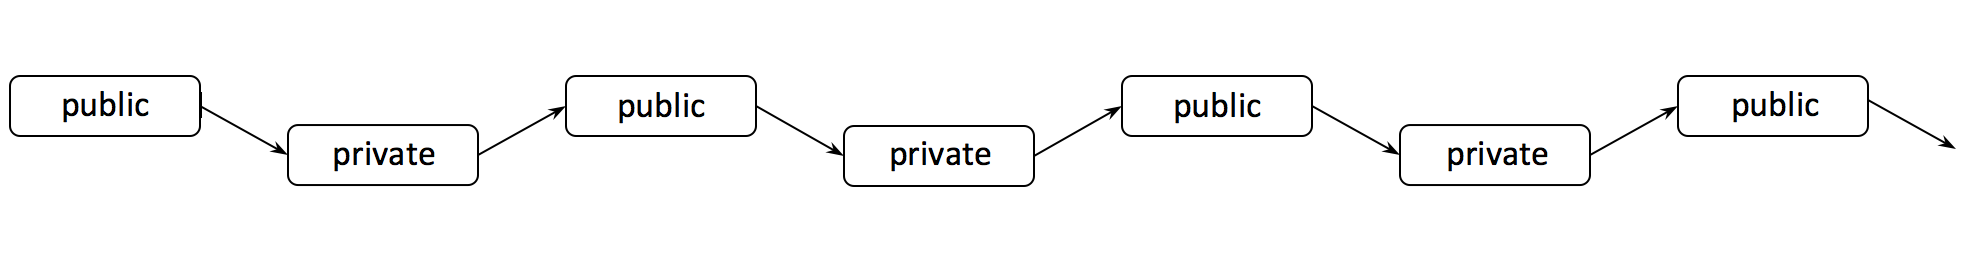
\includegraphics[width=0.9\textwidth,keepaspectratio]{figures/ch02fig01}
\caption{Simplified illustration of iterated practice, or a social 
cognitive causal chain (Sperber 2006:438).}
\end{figure}



Fig. 1 is not the same as the \textquoteleft iterated learning' chains presented by 
Kirby and colleagues (2004; 2008), Christiansen and Chater (2008), among 
others (see below). Those iterated learning depictions resemble Fig. 1, 
but they are not the same. In iterated learning, each arrow from public 
to private may represent an entire learning process in an ontogenetic frame, such as a child's 
learning of a language. Each link in the chain is effectively a single 
macro-level \textquoteleft state change' in ontogeny (e.g., the move from not knowing 
the language to knowing the language). This is shorthand for a great set 
of small events and small associated state changes. 



Learning a language involves not one event but many iterations of 
exposure and reproduction, and in each occasion of exposure and 
reproduction there is feedback that comes from others' reactions to our 
usage of words for communicative goals in context. This feedback plays 
an essential role in learning. Both the microgenetic and ontogenetic frames are relevant. The iterated learning model abstracts 
away from these details (not without practical reason), while the 
iterated practice model in Fig. 1 attempts to capture them directly and 
explicitly. 



While iterated learning focuses on the ontogenetic or biographical 
timescale, iterated practice focuses on the \textsc{enchronic} 
timescale, that is, the timescale of moves and counter-moves in 
sequences of human interaction (Enfield 2009:10; Enfield 2011:285-291, 
2013 Ch. 4). In Fig. 1, each link in the chain from 
private-public-private does not represent a generation of individuals in 
a human population (by contrast with the comparable figure in 
Christiansen and Chater 2008). It represents a generation of individuals 
in a population of \textsc{items}, that is, one local cycle of 
instantiation of a practice, such as a single use of a word, a single 
performance of a ritual, or a single occasion of making bacon and eggs 
for breakfast. 



The schema in Fig. 1 draws our attention to a set of bridges that a bit 
of culture has to cross if it is to survive a cycled of iterated 
practice. What are the forces that facilitate the passage across those 
bridges, and what are the forces that inhibit it? These forces are 
called transmission biases (following Boyd and Richerson 1985; 2005). 
This kind of account assumes a standard model of Darwinian 
evolution---variation of heritable characters in a population---but where 
the variation is guided in a specific way. 



As Boyd and Richerson (1985) formulate it, variation of cultural items 
is guided by the properties of human agents. If, for example, a certain 
way of doing something is easier to learn than some other functionally 
equivalent way (e.g., doing mathematics on a calculator versus on an abacus), 
then this greater ease is likely to increase the frequency of the easier 
variant in the population, and, all things being equal, this variant 
will also in turn increase in frequency simply because it is already 
higher in frequency. 



Christiansen and Chater (2008) use this idea in arguing that the 
properties of the human brain, e.g., for language learning and 
processing, favour certain linguistic variants over others, leading to 
the view that language is the way it is because it is \textquoteleft shaped by the 
brain', and thus not because the evolution of a language faculty has 
caused the human brain to change in some fundamental way as a result of 
the way language is. 



Assuming this model of guided variation, the question then becomes: What 
are the forces that serve to guide variation in this way, and that 
operate upon different variants within a population, ultimately 
determining whether they become, or remain, conventional in the 
population? We now consider some of the known biases.



\section{Some previously described transmission biases}


Variants of cultural behaviour compete for adoption by individuals in 
human populations. Different researchers have described different 
biases, sometimes in quite specific terms, sometimes in broader terms. 



Christiansen and Chater (2008; see also Chater and Christiansen 2010) 
describe four factors that mostly have to do with properties of the 
individual human body, especially the brain. These are (1) perceptuo-motor 
factors, (2) cognitive limitations on learning and processing, (3) 
constraints from mental representations, (4) pragmatic constraints. 
These factors can affect the likelihood that one linguistic variant is 
selected over another, though the social mechanisms that are also a 
necessary part of the process are left implicit by these authors. 



By contrast, Boyd and Richerson (1985) introduce distinctions that are 
broader in kind. They illustrate with an example from table tennis. For 
the function of hitting the ball, one may choose between holding the bat 
with a pencil grip or a handle grip. Choosing one of these variants 
necessary precludes choosing the other. They discuss different biases 
that might cause a person to select one grip over the other. 



A \textsc{direct bias }concerns the relationship between the variant 
and the adopter, and thus it concerns affordances (Gibson 1979). An 
individual should choose variant A if it is somehow more advantageous 
than variant B for a proximate function in a given context. Thus, by a 
direct bias we should choose the grip that is easier, more effective, 
feels better, gives better results. 



An \textsc{indirect bias} works with reference to a notion of social 
identity, assuming that the variant a person selects will be seen by 
others and that this will lend a certain status to both the adopter (as 
the kind of person who adopts that variant) and the variant (as a 
variant that is adopted by that person or someone like that). We adopt 
variants of behaviours not only for their proximate efficacy but also 
with some notion of how we will be seen by others when we make that 
choice. So by an indirect bias we should choose the same grip as people 
who we identify with, or want to emulate. 



Finally, a \textsc{frequency-dependent bias} favours variants that are 
more frequent. 



Similar biases have been described in a vast literature in sociology on 
the diffusion of innovations (Rogers 2003). Here, we can discern three 
sets of conditioning or causal factors in the success or failure of a 
practice. 



First, \textsc{sociometric factors} concern the network structure of 
demographic groups. Different individuals are differently socially 
connected, especially in terms of the number of their points of 
connection to others in a social network, as well as the quality (e.g., 
intensity) of these connections. A practice is more likely to spread if 
it is being modelled by someone who is widely connected in a network, 
simply because he or she will expose a greater number of people to the 
practice. Gladwell (2000) refers to this as the law of the few. 



Second, \textsc{personality factors} concern differences between 
individuals in the population that can have consequences for the success 
or failure of an innovation. Some people are more willing than others to 
innovate and to adopt others' innovations (early adopters versus 
laggards). And these differences may correlate with social categories 
such as age, class, and sub-culture. Some people are better known or 
better admired in their social milieu and may thus be more likely to be 
imitated. 



Third, there is the sheer \textsc{utility} of an innovation, more or 
less what Boyd and Richerson (1985) refer to as direct bias, outlined 
above. The innovation will take off if it is more advantageous to 
potential adopters. 



The biases that we have just reviewed might be seen as a somewhat 
unstructured, ad hoc list. It is clear that they each play an important 
role in the mechanisms of transmission that drive the circulation of 
bits of culture in human populations. But how to explain them? Where do 
these biases come from and how are they related to each other? How can 
we limit this possibility space? Can we motivate these biases by 
locating them directly in the causal anatomy of transmission? What 
predictions are possible? 



One way to motivate and constrain the possibility space of transmission 
biases is to develop an explanatory framework that is grounded in the 
basic structure of iterated practice shown in Fig. 1. Let us now see how 
this structure gives us a way of locating and characterizing the biases. 
If we examine the elements of transmission illustrated in Fig. 1, we see 
at the heart of it a repeating, four-stroke cycle of transmission 
consisting of the following steps: 


\begin{list}{}{}
\item 
(1) \textbf{Exposure}, a process of going from public to private, 
made possible by a mind and body coming into contact with, and 
perceiving/engaging with, the public instantiation of a bit of culture;



(2) \textbf{Representation}, the storing and organizing of a private 
construct based on (1), and the private product of this process;



(3) \textbf{Reproduction}, a process of going from private to public, 
made possible in part by an individual's motivation to cause the same 
public event as in (1). 



(4) \textbf{Material}, the material instantiation of the result of an 
event of reproduction of a cultural item.



(5) Stages (3-4) can then lead to another round by exposing another 
person to the cultural item in question (feeding into a new stage (1)). 

\end{list}





\begin{figure}[h!]
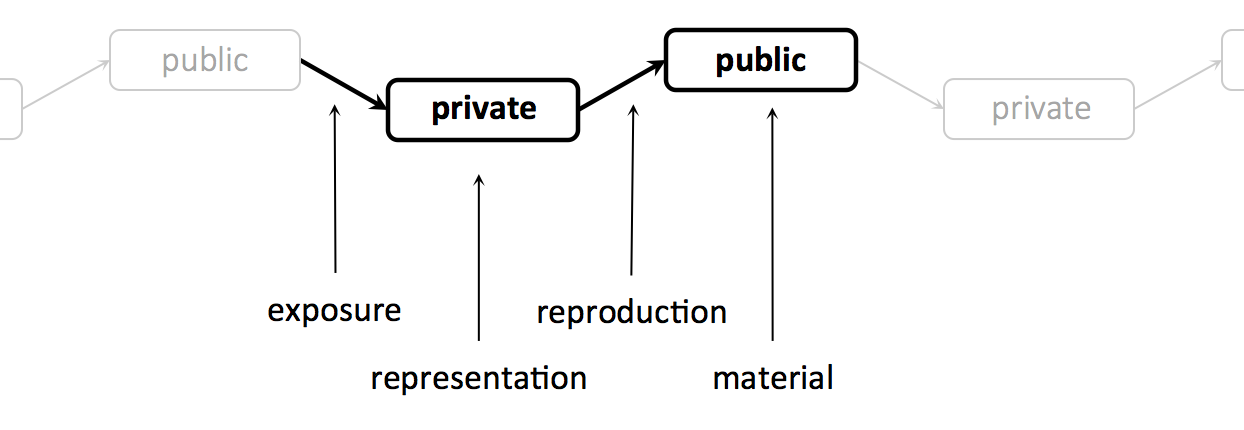
\includegraphics[width=0.9\textwidth,keepaspectratio]{figures/ch02fig02}
\caption{Loci for transmission biases; a four-stroke engine model.}
\end{figure}




Each of the four steps is a bridge or existential threshold for any bit 
of culture to succeed or fail in the competition for uptake in a human 
population. If people aren't exposed to it, it will die. If it is 
difficult to represent mentally, or if in the course of mental 
representation it is radically altered, it will die, or effectively die. 
If people aren't motivated to reproduce it, no further exposure will 
happen, and with the biological death of those individuals who have 
mental representations of the practice in question will come the 
historical death of the practice, as happens for example with language 
extinction. And if the material realization of the practice is not 
available to the perception of others, the transmission process will 
stall. 



Failure on any of these four loci of transmission causes a break in the 
chain and may cause the variant to no longer exist. 



It is important not to get the impression that a single such chain 
represents the entire historical trajectory of a cultural item. It is 
only the tiniest strand. At any moment, there is a thicket of equivalent 
chains of iterated practice that keep a practice alive and evolving in 
the kind of sizable human population that would constitute a historical 
cultural community. 



As discussed above, the key question that a biased transmission approach 
to linguistic epidemiology seeks to answer is: What are the filters, 
pumps, and transformers in an item's career? On the present proposal, we 
can posit four functionally-defined loci at which any bias may have an 
effect. Each locus is defined by the function it serves in accelerating, 
braking, or altering the transmission of practices in human populations 
through social-cultural interaction (i.e., at an enchronic level). 



While there may be a long, if not open list of possible biases, they all 
should be definable in terms of how they operate upon one of the four 
transmission loci, exhaustively defined by the basic causal structure 
represented in Fig. 1 and 2 above: exposure (world-to-mind transition), 
representation (mind structure), reproduction (mind-to-world 
transition), and material (world structure). Within the framework of 
these basic causal loci for transmission (1-4), different specific 
biases may affect the transmission of a practice in qualitatively 
different ways. 



As sketched above, some of these biases will have to do with facts about 
social networks, some with individual personality traits, some with 
properties of human perception, attention, memory, and action, some with 
the shape of the human body, some with the culture-specific means and 
ends that come with culturally evolved structures of activity, some with 
the organization of complex information in cognition. Let us now briefly 
consider how some of the previously described specific biases fit within 
the framework of these minimal loci for cultural transmission.



\textbf{Exposure }(relating to the world-to-mind transition); where 
biases can affect the likelihood that a person will come into contact 
with, and pay attention to, the practice.



\textit{Connectedness.} All people are situated in social networks, 
but they are situated in different ways. One type of difference between 
people concerns the number of other people we come into contact with. 
So-called connectors have a large number of social ties (Granovetter 
1973), and so are more likely to be involved in an encounter with an 
innovation. Those who have few social network connections will have a 
lower chance of being exposed to a given practice. 



\textit{Salience. }Once one is in the presence of a behaviour or kind 
of innovation one may or may not pay attention to it. Things that stand 
out are more likely to be attended to. The definition of \textquoteleft stand out' is 
clearly a matter of perception in the classical sense of affordances, 
that is, a matter of the relationship between a person and the practice. 
Some things are more likely to be noticed because of the nature of our 
perceptual apparatus in relation to the world. Other things are more 
salient to us because we are on the lookout for them, often because our 
language or culture encourages or requires it.



\textit{Identity}. Who is the person carrying out the practice when 
it is encountered? If it is somebody who I want to \textquoteleft be like' in some 
way, then I am more likely to pay attention to what the person is doing 
and how. If it is someone I have no affinity with, or desire to imitate, 
I will be less likely to inspect their behaviour. In this way, social 
identity can play a role in exposure biases, by affecting the extent to 
which someone will attend, or carefully attend, to the practice when 
encountered.



\textbf{Representation }(relating to mind structure); where biases can 
affect the likelihood that, or the manner in which, a practice will be 
learnt or stored by a person, or how the psychological or otherwise 
private component of a practice will be structured. 



Once we have come into contact and at least noticed a practice, we can 
learn it. We form a representation of it, attributing to it some meaning 
or function, and we incorporate that representation in a framework of 
existing representations or knowledge. 



Some innovations are more memorable than others. Of two things we may 
notice, one will be more easily internalized. The reasons for this 
difference concern cognitive propensities that are either known from 
psychological science or that are on that research agenda. 



There are other differences in how things are learnt. The modality of an 
input (seen, heard, felt, or some combination of these) can have 
consequences for how a thing is interpreted, learnt and understood 
(Enfield 2005). This then affects in turn how the knowledge is used in 
practice (e.g., it may account for how an agent decides that a practice 
is an appropriate means for certain ends in a particular context). 



There are effects of the psychological context into which a practice is 
embedded. Practices are partly constituted by knowledge; knowledge that 
is caused by, and in turn causes, public behaviour and associated states 
of affairs. Like any structured domain, knowledge is characterized by 
structured patterns that include part-whole relations, hierarchical 
relations, and other sorts of dependency among items in a system. 



When we learn something, we relate it to other things we know, at the 
very least because the thing was related to other things in the context 
in which we learnt it. As an example, if I learn a new word such as 
\textit{deplane}, I relate it to other words I already know, both in 
terms of similarity (\textit{debone, derail, decode, decommission}) 
and association (e.g., the fact that \textit{deplane} is a verb and 
can be used only with specific grammatical roles in English sentences). 
Or if I learn about the possibility of downloadable ringtones I will 
naturally contextualize this in terms of my existing knowledge of mobile 
phones and the Internet. Through a context bias I am more readily able 
to learn and psychologically represent those things that have an 
existing \textquoteleft place' in which to fit. 



In language, items are structured into conceptual frames, systems of 
categorization, semplates, conceptual metaphors, structural paradigms 
and syntagms. While these systems often display a degree of symmetry, 
consistency, and simplicity, change is always taking place. 



It is in the nature of systems that when something happens in one place 
it will have effects in another place. In the densely structured 
linguistic systems of lexicon and grammar, such system-internal 
relational perturbations sometimes give rise to a certain \textquoteleft psychological 
shakiness', as Sapir (1921) put it, which can lead to reorganization of 
a system, in the private, mental realm, and then potentially in the 
public realm.



In the broadest sense of meaning, capturing everything from the 
arbitrary meanings of words in languages to the affordance-grounded 
functions of tools (Kockelman 2006), we benefit from what can be called 
natural meaning. If a word or grammatical expression is compatible with 
other information, for example by having iconic properties, it is better 
learnt and remembered. 



Similarly for technology, if there is a good match between affordances 
and functions, then we are more likely to understand the practice, it 
will be easier to learn, and indeed what needs to be stored 
representationally is reduced because the relevant information can 
stored materially (Norman 1991). 



This kind of \textit{content bias} pertains to learning, storage, and 
reduction of load on cognition, thus illustrating some ways in which 
'representation' is a functional locus for transmission biases, both in 
language and in culture more generally.



\textbf{Reproduction} (relating to the mind-to-world transition); 
where biases can affect the likelihood that a person will employ the 
practice themselves.



One way to think of this sense of reproduction is whatever causes a 
person to turn the private representation of a practice into action 
whose production and effects are then perceptible by others.



What motivates us to turn knowledge into action? Daily life involves 
goal-directed behaviour that is motivated by our beliefs and desires 
(see e.g., Davidson 2006; Searle 1983; Fodor 1987). I may want to get 
something done for which I need another person's cooperation. One way to 
secure this is to produce an utterance using some selection of words and 
grammatical constructions. Depending on my specific goals, I will select 
certain words and will thereby select against all the other words I 
could have chosen. 



This is the competition among words and grammatical forms invoked in 
Darwin's (1859)(1871:60) quote of Max M�ller (1870): \textquoteleft A struggle for 
life is constantly going on amongst the words and grammatical forms in 
each language'. The competition among different cultural practices 
operates in the same way. I have a goal, I have certain beliefs about 
how it can be attained, I have certain knowledge that allows me to set 
courses of action in motion where certain effects are foreseen. All this 
points to a powerful bias under the reproduction rubric, concerning 
functional needs, and means to ends. 



Boyd and Richerson's \textit{content bias} fits partly under this 
rubric. As discussed above, a content bias favours a practice that is 
more beneficial in some way to the one selecting it. As Boyd and 
Richerson point out, some aspects of these biases are \textquoteleft direct', others 
are \textquoteleft indirect'. A direct bias is in operation when the benefit concerns 
the greater functional payoff, or reduced cost, of the practice, in 
terms of the primary effects it brings about. 



In the table tennis example, a direct bias would favour the pencil grip 
if the pencil grip were lower in cost or greater in benefit than the 
handle grip, that is, in terms of its efficacy for getting the ball back 
over the net and, ultimately, winning matches. An indirect bias is about 
the effects of whom you identify with (or against) by virtue of choosing 
a practice. 



In language, there is an extensive literature on this phenomenon in the 
field of sociolinguistics. Speaking English, I might say \textit{guy} 
in one context and \textit{bloke} in another. It may be that there is 
a slight meaning difference between these two words (thus invoking a 
direct content bias), but these differences may be minimal compared to 
the effect of identifying myself with certain sub-cultural groups or 
kinds of social relationship by virtue of this choice between different 
word forms with near-identical meanings. 



Clearer examples concern pronunciation: whether I choose to say \textit{
working} or \textit{workin'} has more to do with who I identify with 
(an indirect bias) rather than what meaning I want to convey (a direct 
bias). In the cultural realm, both a Rolex and a Tagheuer will tell the 
time for a high price but the choice may depend on whether you want to 
identify with Roger Federer versus Tiger Woods (or, indeed, tennis 
versus golf). 



And there is perhaps most often some combination of the two. Do I choose 
to drink this brand of beer over all the rest because it tastes better 
(a direct bias) or because by doing so I identify with some person or 
group of people (an indirect bias)? It could be both. In any case, the 
mechanisms at play will serve to bias a person's motivation for 
selecting one practice over all the others that he thereby does not 
select. 



The indirect bias is also sometimes described as a \textit{model bias}
. There is an important distinction to be made here depending on the age 
of the person concerned. How does a child select which variants of a 
practice to adopt? A conformity bias favours those practices that 
'everyone else' adopts (Boyd and Richerson 1985; Gergely and Csibra 
2006). 



Another term for this bias is docility (Simon 1990), that is, an 
adaptive propensity to do more or less unquestioningly what other 
members of your group do. For the infant this group will tend also to 
consist of the people to whom one is genetically most closely related. 
The effect is that cultural practices tend to (but need not) have 
similar histories as genes. 



As a person becomes socialized to the point that they are regarded a 
full member of a cultural group, they will encounter a greater range and 
number of cultural items (i.e., they continue learning), and they may 
find themselves therefore with new choices. This may be because they 
encounter other ways of doing things than the way \textquoteleft my people' do things, 
through their contacts with other groups, for instance in trading, 
ritual and other kinds of inter-group social interaction. Different 
people will have different degrees of mobility, sometimes as a result of 
personality, sometimes as a result of gender (men often travel more 
widely than women), age or sub-culture. 



At a later age, there is a greater degree of choice and therefore 
greater competition between choices. We may or may not consciously 
deliberate about such choices. But as adults we may be more aware of the 
meanings of the different options. Here's where the indirect bias looks 
more like the model bias exploited in advertising and also active in any 
other diffusional process as a low-level favouring of those practices 
that are modelled by more admired or charismatic people.



\textbf{Material} (relating to world structure); where biases can 
affect the manner in which a practice will be instantiated in the 
perceptible world. 



Material biases concern the affordances of a cultural item for exposure 
and reproduction. Material biases can affect exposure biases in some 
obvious ways. Speech, for instance, as a result of a particular 
reproduction process (vocalization), has the property of being 
instantiated in fleeting form. A fact about the material of speech is 
that it is perceptible at the time of production but then it is gone. 
But when a reproduction process involving language is carried out 
through writing, this evanescence is dramatically lessened, and the 
dynamics of transmission are significantly affected. 



Outside of language, we see similar contrasts. Forms of activity such as 
adopting a certain grip for table tennis are temporally fleeting and are 
only available for exposure simultaneously with the reproduction process 
that potentially constitutes the transmission event (photos, etc., 
aside). The table tennis bat itself, however, has a more persistent 
physical existence. 



Material biases concern the specific nature of the \textquoteleft publication' of 
cultural practices such that they may continue to play a role in the 
exposure-reproduction cycle described above under the rubric of iterated 
practice.



\section{Conclusion}


The purpose of this chapter has been to address the need for an 
explanatory framework in the study of transmission biases in the ontology of language, with linguistic reality as a case of cultural 
epidemiology more generally. A proper account 
of the cultural evolution of language must be explicit about the causal 
anatomy of the process. Previous work has usefully identified and 
described transmission biases, but one might ask: Why these biases? What 
other biases might we predict are possible? How many might there be? 



We can answer these questions with reference to the basic 
causal anatomy of social transmission in human populations. Cultural 
epidemiology is powered by a four-stroke engine, a causal chain in the enchronic frame from 
exposure to representation to replication to material instantiation, 
back to exposure and round again. When we talk about transmission 
biases, we mean any force that serves as a filter or pump for this 
process, by virtue of its effects on any of the links in this 
potentially open-ended chain of iterated practice. 



Subsequent research should now turn to the tasks of, firstly, seeing if 
we can account for all of the currently known and understood biases 
within this four-stroke engine framework, and secondly, articulating 
predictions made by the framework such that we may empirically test 
them. In addition, such research should ultimately connect to research 
on the initial evolution in our species of the capacity for cumulative 
culture, a capacity that is so strongly pronounced in humans and so weak 
if present at all in our closest relatives the other apes. 



A first place to look for clues would be to consider the known biases in 
connection with what is known about the cognition and social structure 
of other species. While we can readily assume that other animals are 
engaged in goal-directed courses of action, and that they select from 
among different means for certain ends in both the social and material 
realms, their selection of means for ends is relatively less flexible 
than that of humans. 



We might assume that a chimpanzee, say, will be guided in its selection 
of a behavioural strategy by a strong content bias, incorporating a 
basic min-max payoff logic. But if its repertoire of strategies is, on 
the whole, not being acquired by learning from others, then transmission 
biases will have no traction. That said, a topic for research could be 
to look and see the extent to which other apes possess the cognitive 
prerequisites for social transmission of the kind described here. 



While the biggest differences between us and them are known to be in 
social cognition, they are nevertheless intensely social species with 
textured social worlds. Many of the key cognitive and sociometric 
ingredients for biased transmission may have been in place before the 
evolution of our species, allowing the processes to kick in as soon as 
culture was being transmitted at all. 




***
***
NOTES FOR CHAPTER ON DIFFUSION

‘Point of exposure’ - physical path of idea 

The physical path of an idea may (theoretically) be mapped - for this, we may turn to ‘networks’ (Luce 1950, Miller 1951:Ch. 12, Milroy 1980, Ross 1997).

Low density network vs. High density network
	Social networks are not isolated or self-contained, and people in different identified groups may nevertheless maintain ongoing social association. Leach: ‘there is implicit in [relations between human beings in adjacent areas of the map] a social structure’ (Leach 1964:17):


Motivation to infer and create the idea, and to put it into practice

Ideas of all kinds become fashions when a ‘tipping point’ is reached (Gladwell 2000, other works in sociology). This is an exponential acceleration in diffusion of an idea. (How far does a sheet of paper folded 50 times stretch? Why do movie and music producers pour money into potential flops?) Sociology and market research show that in fashion and other social epidemics, the large-scale ‘tip’ hinges directly on \textit{the law of the few} (Gladwell 2000): 

‘Connectors’ Many looser social connections, in a range of social spheres;
‘Mavens’ Informed, interested in the market, want to share that knowledge;
‘Salesmen’ Charismatic, persuasive, set good examples;
‘Innovators’ Experimenters - followed by early adopters, early majority, late majority, laggards.

A select few, of certain \textit{kinds}, are the ones pivotal in epidemics tipping (cf. Gladwell on Paul Revere). The ideas apply directly to linguistic change.

It is recognised that individual responses differ with reference to social function/circumstances (e.g. lifestyle, rank, gender, sociocultural rules, etc.). However, the usual empirically determined categories must be given added texture with the parameter of \textit{personality}.

Adoption of idea 
	- Once exposed, do you or do you not create a representation? 
	- Are you paying attention? Why (not)?
	- What is your emotional response, and will this help you to remember this?
	- What is personally invested in this encounter? 


Reproduction of the behaviour 
	- Will you take the risk of reproducing that behaviour? (What sort of a person are you considered to be?)
	- On what level is that decision made? (conscious/unconscious).
	- To what degree is your representation/reproduction transformed by your subjective intelligence (i.e. the idea takes on attributed semantics \textit{and }social ‘meaning’, which includes what is at stake in which contexts, what \textit{identity} relations) - you don’t ‘catch’ something, you create it yourself.



The risks and rewards of social association impact directly on (and are mediated by) our emotions; this helps to account for our MOTIVATIONS, especially in calculating risk of innovative behaviour (memory is highly geared to emotion); 

Saying things not only communicates a certain meaning in a certain context, but it also advertises \textit{ideas} not only for ‘ways of saying things’, but also ‘things to say’ (cf. Dennett 1995 on technology).

On these bases, I contend that \textit{speakers take an active role in linguistic change of all kinds, including diffusion}. Diffusion results entirely from the decisions individuals make as members of a group, in combination with the principles of \textit{tip}, and the ‘epidemics’ that result. 

True reconstruction of the historical process probably a hopeless quest (Leach quote - history is not ‘irrelevant’, but ‘too difficult to put on paper’.)

 ‘The language’ is one of the basic units of analysis in historical and areal linguistics, and yet this idea is apparently impossible to formally define. (The much more tangible notion of ‘idiolect’ is hardly ever mentioned.)


\textit{better summary than above:
}Linguists know that \textquoteleft a language' is a highly problematic notion, yet we all continue as if it is okay, following native intuitions. But the causal unit of analysis cannot be \textquoteleft the language' - such a category is an IMAGINED one. It is an idea constructed abstractly by linguists and speakers (although for the latter it is less complete, and defined by salient diagnostics). 

Social networks

A model for describing the reality of language in its social context is the network model, pioneered by Milroy (1980), and also taken up more recently by Le Page and Tabouret-Keller (1985), Ross (1997), and others. Ross has recently applied social network theory in modelling sociolinguistic history, towards linguistic and social reconstruction. 
	Milroy (1980) developed a research methodology for studying linguistic variation based around the idea of social networks, ‘the informal social relationships contracted by an individual’ (1980:174), which ‘can be used to account for variability in \textit{individual }linguistic behaviour in communities’ (1980:21). The social network model ‘treats speakers as nodes in a social network, such that each speaker is connected with other speakers by social (and therefore communication) links’ (Ross 1997:213). The idea is to map plot the network of contacts each individual has. Milroy suggested that networks could be placed on a scale of density, from low to high. In a low density network, \textit{a} may be in regular contact with \textit{b}, \textit{c}, and \textit{d}, but \textit{b}, \textit{c}, and \textit{d} are never in contact with each other, while in a high density network, \textit{a}, \textit{b}, \textit{c}, and \textit{d} are all in contact with each other (see diagrams above).

It is also important to note that it is often if not usually the case that contacts between two people are made in the presence of other network-linked participants. Thus, to the ‘High density network’, we could add the ties \textit{a-b-c, a-b-d, a-c-d, b-c-d, }and \textit{a-b-c-d}.

Of the network concept, Milroy writes, ‘its major contribution is to analysis of the manner in which individuals utilise the resources of linguistic variability available to them.’ (1980:175) More recently, in work with Li on the topic of code-switching, she has written:

(A) network analysis can... form an important component in an integrated social theory of language choice. It links the community with the interactional level in focusing on everyday behaviour of social actors...  The link with the economic and sociopolitical level derives from the observation that networks seem to form not arbitrarily but in response to social and economic pressures. (Milroy and Li 1995:155)

Alongside the scale of ‘density’, which refers to the intensity of contact among a given set of network members, further distinctions have been made with regard to the \textit{nature} of the relationship between any two network members. A distinction between ‘exchange’ and ‘interactive’ networks was suggested by Milardo (1988), to which Milroy and Li add ‘passive’ network ties:

	\begin{quotation}
	Exchange networks constitute persons such as kin and close friends with whom ego not only interacts routinely, but also exchanges direct aid, advice, criticism, and support; such ties may therefore be described as ‘strong’.  Interactive networks on the other hand consist of persons with whom ego interacts frequently and perhaps over prolonged periods of time, but on whom ego does not rely for personal favours and other material or symbolic resources; such ties may be therefore described as ‘weak’. An example of an interactive tie would be that between a shop-owner and a customer. In addition to exchange and interactive ties, we identified a ‘passive’ type of network tie, which seemed particularly important to migrant families. Passive ties entail an absence of regular contact, but are valued by ego as a source of influence and moral support. Examples are physically distant relatives or friends. (Milroy and Li 1995:138-9)

	\end{quotation}
\textit{Also add Malcolm Ross on this; or already in fn? insert into main text}

 

\newpage
